\documentclass[10pt,a4paper]{article}

\usepackage[italian]{babel}
\usepackage{amsmath}
\usepackage{amsfonts}
\usepackage{amssymb}

\usepackage[left=1cm,right=1cm,top=1cm,bottom=2cm]{geometry}

\usepackage{txfonts}
\usepackage[T1]{fontenc}
\usepackage[utf8]{inputenc}

\usepackage{titlesec}
\setcounter{secnumdepth}{4}
\titleformat{\paragraph}{\normalfont\normalsize\bfseries}{\theparagraph}{1em}{}
\titlespacing*{\paragraph}{0pt}{3.25ex plus 1ex minus .2ex}{1.5ex plus .2ex}

\usepackage{graphicx}
\usepackage{subcaption}

\usepackage{wrapfig}

\usepackage{siunitx}

\pagenumbering{arabic}
\pagestyle{plain}

% per non farlo anadre a capo ovunque
\usepackage[none]{hyphenat}
% per togliere gli ident all'inizio dei paragrafi
\setlength{\parindent}{0pt}


\begin{document}
\subsection{Il computo parallelo}
L'incremento di prestazioni dei calcolatori fa sempre più affidamento all'ausilio delle GPU, le quali vengono utilizzate sempre di più per operazioni non prettamente grafiche, le quali presentano un' architettura che punta alla massimizzazione del numero di unità di elaborazione e non più all'incremento della frequenza di lavoro.\\
Tale approccio non è sempre il migliore, infatti la loro efficacia è strettamente legata al tipo di applicazioni, in particolare alla parallelizzabilità del codice, ovvero alla dipendenza di determinate istruzioni di avere a disposizione i dati elaborati da istruzioni precedenti.\\
Questa architettura trova la massima efficacia quando un grande numero di istruzioni è completamente indipendente dalle altre. 

\begin{figure}[h!]
  \centering
  \begin{subfigure}[t]{0.45\linewidth}
  	\centering
    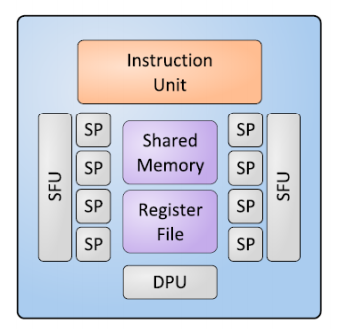
\includegraphics[height=200pt]{SM.PNG}
    \caption*{Struttura di uno stream-multiprocessor}
  \end{subfigure}
  \begin{subfigure}[t]{0.45\linewidth}
  	\centering
    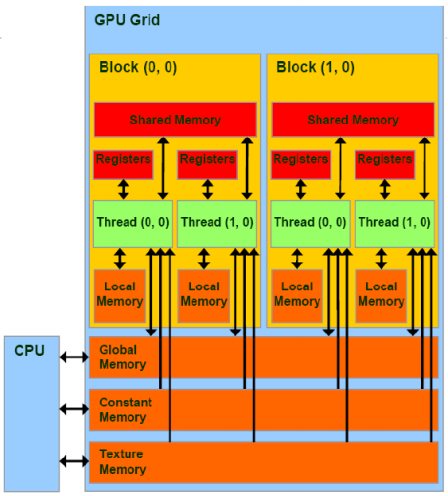
\includegraphics[height=200pt]{LogicModel.PNG}
    \caption*{Struttura logica della GPU}
  \end{subfigure}
  \label{fig:graph1}
\end{figure}

\subsubsection{L'architettura della GPU}
La struttura della GPU è definita "SIMT" (single instruction, multiple thread), tale aggettivo è dato in quanto la GPU è realizzata per eseguire un medesimo programma su un gran numero di processori contemporaneamente, i quali però ricevono dati diversi da computare.\\ Tipicamente i processori presenti su una GPU sono più piccoli e semplici di quelli di una CPU e anche molto meno performanti ma il loro grande numero e la strutturazione delle memorie presenti al suo interno permette per il codice parallelizzabile di ottenere tempi di esecuzione estremamente minori rispetto a quelli in una CPU.\\
Uno dei componenti più importanti in una GPU è lo stream-multiprocessor, Il quale  può essere considerato un processore vettoriale, una GPU solitamente ne contiene diversi, e compongono il modello fisico della GPU, i quali a loro volta sono composti principalmente da tre  unità di calcolo: 

\begin{itemize}
  \item \textbf{SP (scalar processor)} - E' un'unita logica che esegue operazioni in virgola fissa e mobile di un solo thread per volta, è inportante inoltre sapere che gli SP di uno stesso SM hanno una memoria detta shared condivisa che gli permette di scambiarsi dati con estrema velocità a tempo di esecuzione.
  \item \textbf{SFU (special functions unit)} - E' un'unità logica di supporto agli SP che esegue a livello HW funzioni complesse come le funzioni gognometriche e trascendenti che appesantirebbero eccessivamente gli SP.
  \item \textbf{DPU (double proces unit)} - Quest'ultima si occupa delle operazioni su numeri a 64 bit, i double.
\end{itemize}

Una delle peculiarità più importanti della GPU è la differenza tra il modello fisico e quello logico, infatti il modello al quale il programmatore deve far riferimento per ottimizzare l'esecuzione del codice è una via di mezzo tra quello logico e quello che la macchina implementa fisicamente, cercando il bilanciamento migliore possibile tra comprensibilità dei dati e ottimizzazione del codice.
Il modello logico. Il programmatore infatti ha la possibilità di interagire e modellare questa struttura composta da oggetti logici detti griglie (GRID), tali griglie possono avere tre dimensioni e a loro a volta sono composte da altri oggetti logici detti blocchi, i quali possono avere fino a tre dimensioni, che in fine sono composti da thread.
Ogni SM generalmente processa un blocco alla volta, mettendo a disposizione la sua shared memory tra i thread dello stesso blocco, tra i vari blocchi e griglie è possibile lo scambio di informazioni esclusivamente attraverso la global memory, molto più grande delle cache degli SM ma anche molto più lenta. 
Un'ultimo argomento da trattare riguardo il legame tra la struttura logica e quella hardware della GPU è \underline{"il flusso di esecuzione"} ovvero il metodo con cui lo scheduler, ovvero l'organo interno che si occupa della ripartizione delle operazioni ,strutturate dal programmatore nella griglia, ai vari SM. Tale operazione ha come unità base il \underline{warp}, ovvero un numero n dipendente dalla specifica architettura, nel nostro caso 32, di thread appartenenti allo stesso blocco che vengono eseguiti contemporaneamente in maniera "lookstepped" (ovvero in sincronizzazione forzata). L'esecuzione del warp si conclude e si passa al successivo solo nel momento in cui tutti i suoi thread arrivano a fine esecuzione indipendentemente dalla "branch" di programma che hanno seguito.
\\ \\
\subsubsection{L'utilizzo della GPU per il deep-learning}
Nel deep learning come illustrato nella sezione precedente, si effettuano moltissimi calcoli, i quali sono per gran parte scorrelati tra loro, caratteristica questa fondamentale per la parallelizzazione delle operazioni.
L'utilizzo di calcolatori paralleli per l'addestramento delle reti neuronali consente di completare addestramenti per modelli molto grandi in tempi molto ridotti. Confrontando l'addestramento di una rete su una CPU desktop rispetto ad una GPU da gaming si possono incrementare le prestazioni da 200 a 500 volte, ciò significa che un addestramento di un'ora su GPU, può richiedere su una CPU un tempo che può andare da una a tre settimane. \\ \\
(Nel nostro caso da un i5-4670k abbiamo avuto un incremento di prestazioni di 250 volte su una GPU Nvidia gtx760 asus, con un programma che pecca fortemente di ottimizzazione).     
\end{document}